\documentclass[tikz,border=3pt]{standalone}
\usepackage[T1]{fontenc}
\usepackage[utf8]{inputenc}
\usepackage[english]{babel}
\usepackage{mathptmx}
\usepackage[scaled=0.92]{helvet}
\usepackage{amsmath,amssymb,textcomp}
\usetikzlibrary{positioning,arrows.meta}
\newcommand{\us}{\textmu s}
\begin{document}
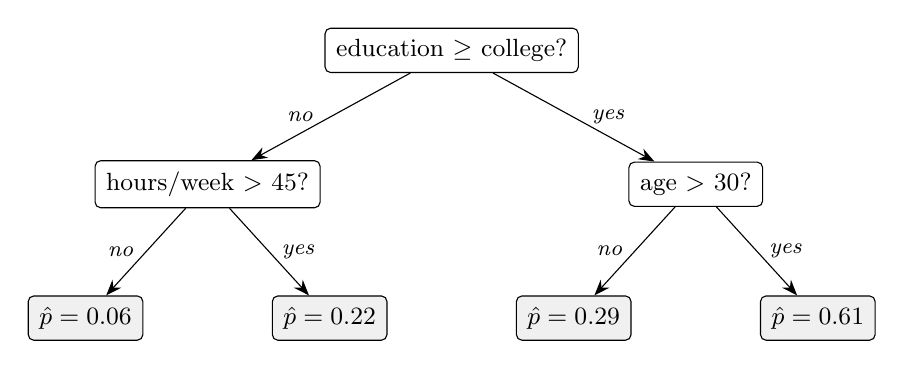
\begin{tikzpicture}[
  level distance=17mm,
  level 1/.style={sibling distance=62mm},
  level 2/.style={sibling distance=31mm},
  interno/.style={draw, rounded corners=2pt, align=center, font=\small,
                  inner sep=4pt},
  folha/.style={draw, rounded corners=2pt, align=center, font=\small,
                fill=black!6, inner sep=4pt},
  rotulo/.style={font=\footnotesize\itshape, midway},
  edge from parent/.style={draw, -{Stealth[length=2mm]}}]
\node[interno] {education $\geq$ college?}
  child { node[interno] {hours/week $>$ 45?}
    child { node[folha] {$\hat{p} = 0.06$}
      edge from parent node[rotulo, left=1pt] {no} }
    child { node[folha] {$\hat{p} = 0.22$}
      edge from parent node[rotulo, right=1pt] {yes} }
    edge from parent node[rotulo, left=3pt] {no} }
  child { node[interno] {age $>$ 30?}
    child { node[folha] {$\hat{p} = 0.29$}
      edge from parent node[rotulo, left=1pt] {no} }
    child { node[folha] {$\hat{p} = 0.61$}
      edge from parent node[rotulo, right=1pt] {yes} }
    edge from parent node[rotulo, right=3pt] {yes} };
\end{tikzpicture}
\end{document}
